\pdfoutput=1
% ^ arXiv: process with pdflatex (must appear in the first five lines).
% Preprint — builds with any standard TeX Live (all packages below are TeX
% Live core; no shell-escape); figures are prebuilt PDFs from make_figures.py.
% Sources of truth: research/decathlon{,2,3,4}.json, research/fx.json,
% research/crypto.json, docs/FINDINGS.md, docs/METHODS.md, docs/design/DESIGN{8,18,20,22}.md.
% Repo convention: no author block in-repo; a byline is added only at submission time.
\documentclass[11pt]{article}
\usepackage[margin=1.15in]{geometry}
\usepackage{amsmath,amssymb}
\usepackage{graphicx}
\usepackage{booktabs}
\usepackage{microtype}
\usepackage[round]{natbib}
\usepackage[hidelinks]{hyperref}
\graphicspath{{figures/}}

% Small captions with a bold "Figure N." label. Standard TeX Live path:
% caption.sty. Fallback for minimal installations that lack caption.sty
% (e.g. bare TinyTeX): an equivalent kernel-level \@makecaption — same
% \small text, same bold label, centered when the caption fits one line.
\makeatletter
\long\def\kronos@makecaption#1#2{%
  \vskip\abovecaptionskip
  \small\sbox\@tempboxa{\textbf{#1.} #2}%
  \ifdim \wd\@tempboxa >\hsize
    {\small\textbf{#1.} #2\par}%
  \else
    \global\@minipagefalse
    \hb@xt@\hsize{\hfil\box\@tempboxa\hfil}%
  \fi
  \vskip\belowcaptionskip}
\IfFileExists{caption.sty}
  {\usepackage[font=small,labelfont=bf,labelsep=period]{caption}}
  {\let\@makecaption\kronos@makecaption}
\makeatother

\newcommand{\cfg}[1]{\mbox{#1}}

\title{Efficiency and Wildness Are Jointly Produced:\\
A Three-Way Refutation in Minimal Market Models}
\author{}
\date{}

\begin{document}
\maketitle

\begin{abstract}
\noindent
Agent-based models reproduce financial stylized facts piecemeal; whether a
single minimal mechanism can buy them all is open. We score minimal flow-based
markets against a ten-event battery calibrated so that real equity data passes
all ten events and geometric Brownian motion exactly three. A market of
fundamentalists, chartists, volatility-targeters and market makers reaches five
of ten, and its failures are diagnostic: the missing events concern long
memory, time-irreversibility, and information-free price signs. We then test,
in three pre-registered experiments with kill criteria, whether rationality can
close the gap: (i) an anticipatory agent that front-runs the forecastable flow;
(ii) the fixed point of mutual anticipation, iterated to depth five; (iii) a
price-setting maker that provably absorbs the forecastable component into the
price level. All three fail, and they fail informatively: deeper anticipation
\emph{grows} the sign leak while contracting the flow it targets, and exact
absorption kills the fat tails, the leverage effect and volatility clustering
along with the leak. We conclude that in this model class, sign-efficiency and
the wild stylized facts are jointly produced by the same state-riding flows and
are not separately purchasable. An empirical counterpart --- the leverage
effect's sign ordered by market microstructure across equities ($-0.04$), FX
($\approx 0$), and crypto ($+0.03$) --- is consistent with the mechanism. All
results are pre-registered, gate-verified against synthetic ground truth, and
regenerable from the public repository.
% src: abstract v1, docs/paper/OUTLINE.md; leverage values research/fx.json leverage_contrast
\par\medskip
\noindent\textit{Keywords:} stylized facts; agent-based markets; market
efficiency; price impact; leverage effect; pre-registered negative results.
\end{abstract}

\section{Introduction}
\label{sec:intro}

Real price series manage two things at once: their return signs are nearly
unforecastable, and their amplitudes are wild --- heavy tails, clustered
volatility, crash asymmetry. This paper asks whether a minimal market
mechanism can buy both properties together, and answers by refutation: in
flow-based minimal markets, sign-efficiency and wildness are jointly produced
by the same flows, and three pre-registered attempts to purchase them
separately --- rationality added as a trading agent, as the fixed point of
mutual anticipation, and as a price-setting rule --- all fail against kill
criteria declared in advance. The refutations are the result: they compose
into a structural claim about what this model class cannot do, measured on a
fixed instrument (Figure~\ref{fig:scorecard}).

The question sits in a literature with a shared target list: the stylized
facts --- heavy tails, volatility clustering, the leverage effect,
near-absence of linear return autocorrelation --- that any candidate mechanism
for price formation should reproduce \citep{cont2001}. Agent-based modeling
took up the challenge early: heterogeneous-agent markets with fundamentalists
and chartists generate fat tails and clustered volatility from agent
interaction rather than from exogenous news \citep{lux1999}, and a substantial
literature has since mapped which ingredients produce which facts
\citep{lebaron2006}. Two gaps in that literature motivate the design here.
First, scoring is usually piecemeal: a model is exhibited that matches two or
three facts, with the remaining facts unexamined, so the literature
accumulates existence proofs rather than a ledger of what a given mechanism
class can and cannot buy. Second, negative results are structurally
underproduced: when an added ingredient fails to improve a model, the failure
is rarely reported, almost never pre-registered, and so carries no evidential
weight. We address both gaps with a fixed measurement instrument and a
pre-registered refutation chain.

\begin{figure}[t]
\centering
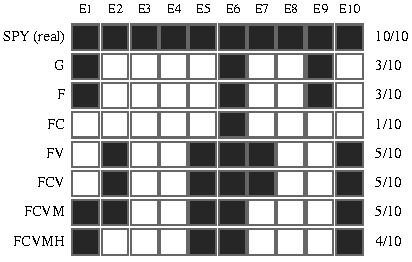
\includegraphics[width=0.72\linewidth]{battery_scorecard}
\caption{Battery scorecard: real SPY against the ablation ladder (filled =
pass). G = noise only (GBM); F adds fundamentalists; C chartists; V
volatility-targeters; M market makers; H multi-horizon heterogeneity. No flow
configuration exceeds 5/10, and the five events missing from the best
configuration (\cfg{FCVM}) are E3, E4, E7, E8, E9.}
% src: research/decathlon.json spy.events, configs.*.events
\label{fig:scorecard}
\end{figure}

\paragraph{Contribution (i): a battery, calibrated at both ends.}
We distill ten events (E1--E10) from a prior measurement program on real
markets --- price efficiency, fat tails, volatility clustering, long memory in
the volatility clock, the leverage effect, conditional Gaussianity given the
volatility path, clock jumps, the arrow of time in the return--volatility
coupling, information-free price signs, and gain/loss tail asymmetry --- each
with a numeric pass criterion fixed before any simulation was run
(Section~\ref{sec:battery}). The battery is calibrated so that real SPY data
passes 10/10 while geometric Brownian motion passes exactly 3/10; this spread
is the instrument's dynamic range, and it is enforced by an automated gate that
runs on every commit.
% src: research/decathlon.json spy.score=10, configs.G.score=3; docs/design/DESIGN8.md (gate X19)

\paragraph{Contribution (ii): a pre-registered refutation arc.}
The best flow-only configuration of a minimal market stalls at 5/10, and the
five missing events are diagnostic: they concern long memory,
time-irreversibility, and the information content of price signs. Three
successive experiments --- each pre-registered with hypotheses, budgets, and
kill criteria before any evaluation run --- then test whether
\emph{rationality} can close the gap: a single anticipatory agent
(Section~\ref{sec:deca2}), the fixed point of mutual anticipation iterated to
depth five (Section~\ref{sec:deca3}), and a price-setting market maker that
absorbs the forecastable flow into the price level by algebraic identity
(Section~\ref{sec:deca4}). All three are refuted, and because each refutation
was armed with a mechanism gate proving the tested agent \emph{works}, the
refutations compose into a structural claim (Section~\ref{sec:structural}):
in this model class, sign-efficiency and the wild stylized facts are jointly
produced by the same state-riding flows and cannot be purchased separately.

\paragraph{Contribution (iii): a methodology that makes negative results evidential.}
Every estimator is licensed by a convict-and-exonerate gate --- it must detect
a planted effect on synthetic data where the effect exists and must stay silent
where it does not --- before it touches evaluation data
(Section~\ref{sec:methods}). Every experiment pre-declares its parameter
budget, its contingent tuning pass, and its tie-break rule; the third
experiment additionally pre-declared a closure clause naming itself the final
attempt on the line. Under this regime a refutation is not an absence of
result; it is a measurement.

The headline mechanism result is easy to state. Adding one layer of
anticipation to the minimal market leaves its score unchanged and moves the
sign leak --- the residual forecastability of next-day return signs, defined
precisely in Section~\ref{sec:battery} --- one derivative earlier; iterating
anticipation five deep contracts
the model-space forecastable flow by a factor of four while the leaked sign
information in the realized prices moves the wrong way (median direction
bits 0.0184 $\to$ 0.0200 $\to$ 0.0257; the depth-five rise holds on 7 of 8
paired seeds); and a maker that removes the
forecastable component's price impact exactly --- verified to the identity on a
toy world --- does not close the leak either, but instead deletes the fat
tails (kurtosis $8.8 \to 3.0$), the leverage effect ($-0.125 \to -0.008$), and
volatility clustering along with the wildness the flows were generating.
% src: research/decathlon3.json dir_bits_vs_K medians; research/decathlon4.json configs FCVM/FCVM+Q1.0 median_stats
Efficiency in signs and wildness in amplitudes are not separate dials in this
model class. Section~\ref{sec:triangle} adds an empirical observation that is
consistent with the mechanism --- the leverage effect's sign across equities,
FX, and crypto is ordered exactly as the flow-structure story predicts ---
without claiming it as proof.

\section{The battery and the base market}
\label{sec:battery}

\subsection{Ten events}

The battery consists of ten binary events, computed identically on real data
and on simulated output, with pass criteria fixed before any agent-based run.
Table~\ref{tab:events} lists them; Appendix~\ref{app:battery} gives the exact
statistic definitions and thresholds as implemented, together with the full
statistic vector at both calibration ends. The events are close-only versions
of regularities measured and gate-validated in a prior program on $\sim$48
liquid US equities and ETFs (2010--2026), so the thresholds are empirical
ranges, not conventions.
% src: docs/design/DESIGN8.md (event table and calibration amendments)

\begin{table}[t]
\centering\small
\begin{tabular}{llp{7.6cm}}
\toprule
\# & Event & Pass criterion \\
\midrule
E1 & price efficiency & AC$_1(r) \in [-0.15, 0.05]$ (allows the real index's mild daily reversal) \\
E2 & fat tails & kurtosis$(r) \in [4.5, 40]$ \\
E3 & vol clustering & AC$_1(|r|) \ge 0.12$ and mean AC$(|r|, \text{lags }5\text{--}20) \ge 0.05$ \\
E4 & long-memory clock & 8-week volatility-clock level autocorrelation above threshold \\
E5 & leverage effect & mean corr$(r_t, \mathrm{RV}_{t+1..10}) \le -0.03$ \\
E6 & one-clock Gaussianization & kurtosis$(r/\sigma_{5d}) \le 5$ \\
E7 & clock jumps & AR(1) clock-innovation skew beyond the log-$\chi^2$ noise floor \\
E8 & arrow of time in the coupling & entropy production significant in $r$ and reduced $\ge 25\%$ by vol deformation \\
E9 & no sign information & direction bits $\le$ shuffle null (95\%) \\
E10 & tail asymmetry & gain/loss tail asymmetry at 2.5$\sigma$ \\
\bottomrule
\end{tabular}
\caption{The ten-event battery (final calibrated form; exact estimator
definitions and thresholds in Appendix~\ref{app:battery}). E1, E4, E7 and E10
were recalibrated against real data before any ablation was run, under a gate
requiring real SPY to score 10/10 and geometric Brownian motion exactly 3/10;
notably, a GJR-GARCH process fails E4 --- exponential memory cannot fake long
memory. E9 measures the mutual information between three public tape features
and the next-day return sign with a discrete plug-in estimator against a
permutation null.}
% src: docs/design/DESIGN8.md events + calibration-phase amendments; kronos/decathlon.py battery()
\label{tab:events}
\end{table}

Calibration pins both ends of the scale: real SPY (close-only) scores 10/10;
a pure GBM scores exactly 3/10, passing only E1, E6 and E9 --- Gaussian worlds
are efficient, trivially one-clock, and carry no sign information. Everything
between 3 and 10 is what a mechanism must buy. Two scoping remarks. The
thresholds are ranges from the multi-asset program, but the joint-10/10
anchor is a single index; the battery's job in this paper is comparative ---
every configuration is scored on the same events with the same seeds --- not
to certify any absolute realism. And a battery score carries no formal
standard error; what protects the comparisons is that they are paired (all
configurations share seeds 100--107) and that every conclusion below rests on
a pre-registered kill criterion, not on a one-event margin.
% src: research/decathlon.json spy.score, configs.G

\subsection{The minimal market}

The base market is deliberately small: aggregated flows, about a dozen
parameters, linear impact. Log price $p_t$ moves by
%
\begin{equation}
r_t \;=\; \lambda\,\bigl[\,D^{\mathrm{fund}}_t + D^{\mathrm{chart}}_t +
D^{\mathrm{vol}}_t + D^{\mathrm{mm}}_t + D^{\mathrm{noise}}_t\,\bigr],
\label{eq:market}
\end{equation}
%
with price-impact coefficient $\lambda$;
$D^{\mathrm{fund}} = k_F\,(V_t - p_t)$ for a random-walk log fundamental $V$;
$D^{\mathrm{chart}} = k_C \tanh(m_t/s)$ for an EWMA trend signal $m$;
$D^{\mathrm{vol}} = k_V\,(L_t - L_{t-1})$ for volatility-targeters (hereafter
vol-targeters) running the
leverage rule $L = \min(L_{\max}, \sigma^{*}/\hat\sigma)$ against an EWMA
variance estimate $\hat\sigma^2$;
a one-lag market-maker flow $D^{\mathrm{mm}} = -k_M\, r_{t-1}$; and i.i.d.\
noise. The volatility-targeting flow is the reflexive ingredient: a vol spike
forces de-leveraging (selling), which moves price, which raises vol. The
market-maker ingredient was added at the calibration stage, before any
ablation was scored, when tuning showed that vol-targeting flows structurally
leak momentum --- their de-leveraging is serially correlated --- and that in
reality such flow is absorbed by liquidity provision.
% src: docs/design/DESIGN8.md (model spec; amendment 2)

Parameters were hand-set once on the full configuration to produce sane
volatility levels and pass E1--E3 only, and were not tuned per configuration
or per event; ablations zero out flows and change nothing else. Eight seeds
per configuration, $T = 6000$; an event passes if a majority of seeds pass.
% src: docs/design/DESIGN8.md honesty constraints

\subsection{The ablation ladder and the 5/10 ceiling}

Figure~\ref{fig:scorecard} shows the ladder. Noise alone (G) and
fundamentalists alone (F) score the Gaussian 3/10. Chartists without
discipline are toxic: \cfg{FC} scores 1/10, because the momentum leak destroys
even efficiency. The vol-targeters are the star ingredient:
\cfg{FV} jumps to 5/10, buying the wild one-sided facts --- fat tails (E2),
the leverage effect (E5), clock jumps (E7), crash asymmetry (E10) --- because
the de-leveraging spiral is the only flow that reacts to volatility and reacts
in one direction only. Adding market makers (\cfg{FCVM}) restores efficiency
(E1) at the cost of E7, holding the score at 5/10: efficiency and wildness are
contributed by \emph{different} agents. Multi-horizon heterogeneity
(\cfg{FCVMH}) fails both ways, dropping to 4/10.
% src: research/decathlon.json configs G/F/FC/FV/FCVM/FCVMH scores+events

\begin{table}[t]
\centering\small
\begin{tabular}{lrrrrr}
\toprule
 & AC$_1(r)$ & kurtosis & AC$_1(|r|)$ & leverage & E9 bits \\
\midrule
SPY (real)        & $-0.103$ & 15.1 & 0.31 & $-0.113$ & 0.0029 \\
GBM (G)           & $0.001$  & 3.0  & $-0.001$ & $0.007$ & 0.0001 \\
\cfg{FCVM} (best flow-only) & $0.036$ & 8.8 & 0.38 & $-0.125$ & 0.0184 \\
\bottomrule
\end{tabular}
\caption{Key medians. \cfg{FCVM} reproduces efficiency, tails, clustering
amplitude and the leverage effect at realistic magnitudes; what it cannot do
is keep the sign channel silent (E9: 0.0184 significant direction bits against
SPY's 0.0029) or generate long memory and the coupling arrow.}
% src: research/decathlon.json spy.stats, configs.G.median_stats, configs.FCVM.median_stats
\label{tab:fcvm}
\end{table}

The ceiling is 5/10 and the five missing events are a diagnosis
(Table~\ref{tab:fcvm}). \cfg{FCVM} fails E3 (slow volatility clustering), E4
(long-memory clock), E7 (clock jumps, marginally), E8 (the arrow in the
coupling), and E9 (information-free signs). The E9 failure is the paper's
through-line, so we give it a name used throughout: the \emph{sign leak} ---
a significant excess of E9's statistic, the \emph{direction bits}
$I(\text{tape features};\, \mathrm{sign}\, r_{t+1})$, over its shuffle null.
\cfg{FCVM} leaks 0.0184 bits where real SPY shows 0.0029. The leak has a
known source: the vol-targeters' de-/re-leveraging drift is serially
correlated and forecastable from the tape, and a one-lag market maker cannot
absorb a multi-day drift. The natural hypothesis --- the one this
paper's arc tests to destruction --- is that the missing organ is
\emph{expectation}: rational agents who anticipate the predictable flow should
arbitrage the sign leak away and perhaps stretch the volatility episodes into
long memory.
% src: docs/design/DESIGN18.md (ceiling diagnosis); research/decathlon.json configs.FCVM

\section{Experiment I: one anticipator}
\label{sec:deca2}

\subsection{Design}

The vol-targeters' flow is mechanical and forecastable from public information
alone: their mandate ($L = \min(L_{\max},\sigma^*/\hat\sigma)$) and their
estimator (an EWMA of squared returns at a known speed) are both computable
from the price tape. The anticipatory agent A is handed exactly that and
nothing else. At each step it reconstructs $\hat\sigma^2_t$ from the return
history, forecasts the integrated future mechanical flow under the one belief
that defines vol-targeting --- volatility reverts to the targeters' own
target, so leverage ends at $L_{\mathrm{eq}} = \min(L_{\max}, 1)$ ---
%
\begin{equation}
\hat F_t \;=\; k_V \cdot \mathrm{mean}_{\mathrm{cohorts}}\bigl(L_{\mathrm{eq}} - L_t\bigr),
\label{eq:forecast}
\end{equation}
%
holds inventory proportional to the forecast, capped by capital,
$I^*_t = \mathrm{clip}(k_A \hat F_t, \pm \mathrm{cap}_A)$, and trades the
inventory change plus execution noise of scale $s_A$. The unwind is automatic:
as vol reverts
and the targeters re-lever, the forecast decays and the anticipator sells into
exactly that mechanical bid. Three parameters
$(k_A, \mathrm{cap}_A, s_A)$ --- response, capital, noise --- frozen before
any battery run.
% src: docs/design/DESIGN18.md (agent spec)

Three gates license the mechanism before any score is read (the pattern is
described in Section~\ref{sec:methods}): (a) with the agent disabled the
simulator reproduces the original market byte-for-byte, protecting the
SPY-10/GBM-3 calibration; (b) the forecast is causal --- tampering with future
returns leaves the trade prefix unchanged; (c) on a deterministic toy world
with a perfectly predictable mechanical flow, the anticipator profits
\emph{and} damps the flow's price impact, from 1.00 to 0.75 per unit of
arriving flow. The agent demonstrably works. The pre-registered kill
criterion: if the frozen configuration does not exceed 5/10 on the evaluation
seeds, the expectation hypothesis is refuted.
% src: docs/design/DESIGN18.md (gates X30a-c, kill criterion); docs/FINDINGS.md DECATHLON-2

The parameter protocol matters for what follows. The first-shot parameters
$(k_A, \mathrm{cap}_A, s_A) = (0.5, 0.02, 0.002)$ scored 4/10 on tuning seeds
disjoint from evaluation, so the single pre-registered grid pass was spent:
its best score was 5/10, tied across all six $k_A = 0.25$ combinations plus
one weak $k_A = 0.5$ setting --- flat wherever the anticipator is weak. The
pre-declared deterministic tie-break (lexicographically smallest, i.e.\ the
weakest anticipator) selected $(0.25, 0.01, 0.001)$. That the selection lands
on ``trade as little as possible'' was recorded, at registration time, as
already being evidence about the hypothesis.
% src: research/decathlon2.json tuning; docs/design/DESIGN18.md amendment

\subsection{Result: refuted, with the leak moved one derivative earlier}

\begin{table}[t]
\centering\small
\begin{tabular}{llll}
\toprule
Config & Score & Failed events & E9 bits (median) \\
\midrule
\cfg{FCVM} (control)      & 5/10 & E3 E4 E7 E8 E9 & 0.0184 \\
\cfg{FCVM+A} (hypothesis) & 5/10 & E3 E4 E7 E8 E9 & 0.0200 \\
\cfg{FV+A}                & 5/10 & E1 E3 E4 E8 E9 & 0.0158 \\
\cfg{F+A} (no targeters)  & 3/10 & $=$ \cfg{F} exactly & 0.0002 \\
\bottomrule
\end{tabular}
\caption{Experiment I ablation (8 evaluation seeds, majority vote). Adding the
anticipator changes nothing that was supposed to change: the failure set is
identical and the direction bits do not fall.}
% src: research/decathlon2.json configs (scores, events, median_stats.dir_bits)
\label{tab:deca2}
\end{table}

Table~\ref{tab:deca2} shows the outcome. The kill criterion fires:
\cfg{FCVM+A} scores 5/10 with a failure set identical to the control's. The
events expectation was supposed to buy did not move --- the direction bits
did not move toward zero (medians $0.0184 \to 0.0200$; the paired per-seed
comparison splits 4--4, so the licensed reading at one layer is
``unchanged,'' not ``reduced''), and the long-memory events stayed flat. The interaction hypothesis held: without vol-targeters the anticipator
buys nothing (\cfg{F+A} $=$ \cfg{F} $=$ 3/10) --- expectation needs a
predictable flow to trade against; it simply does not fix anything when it has
one.
% src: research/decathlon2.json configs; docs/FINDINGS.md DECATHLON-2

Why it fails is the finding. The tuning grid is monotone: the harder the
anticipator trades, the worse the market scores. Efficiency breaks (its unwind
adds reversal: AC$_1$ falls from $-0.09$ toward $-0.35$ as $k_A$ rises), the
tails erode (it damps the very spiral that generates them, kurtosis
$8.8 \to 4.6$), and the sign leak \emph{grows} (up to 0.039 bits at full
strength $k_A = 1$).
% src: docs/FINDINGS.md DECATHLON-2 (tuning-grid mechanism paragraph)
The mechanism is structural, not parametric: the anticipator's inventory is a
function of the same slow public volatility state as the flow it front-runs,
so its own future unwind is exactly as forecastable as what it absorbs. One
layer of expectation does not remove the predictable flow; it reproduces the
leak one derivative earlier, while eating the wildness. The refutation names
its own successor: if one anticipator re-leaks because its inventory is
public-state-driven, perhaps information-free prices require anticipators who
anticipate \emph{each other} --- the fixed point of mutual anticipation.

\section{Experiment II: the fixed point of mutual anticipation}
\label{sec:deca3}

\subsection{The iterated operator and its algebra}

The fixed-point stack makes each layer's unwind part of what is anticipated.
Layer $k$ front-runs the \emph{residual} forecastable total flow --- the
mechanical flow plus the deterministic future unwind of the $k-1$ layers
beneath it (time subscripts suppressed):
%
\begin{equation}
\mathrm{resid}_0 = \hat F, \qquad
J_k = \mathrm{clip}\bigl(k_A\,\mathrm{resid}_{k-1}, \pm \mathrm{cap}_A\bigr), \qquad
\mathrm{resid}_k = \mathrm{resid}_{k-1} - J_k, \qquad
I_K = \textstyle\sum_{k=1}^{K} J_k .
\label{eq:stack}
\end{equation}
%
Away from the caps this telescopes: $I_K = \bigl(1-(1-k_A)^K\bigr)\hat F$, and
the model-implied forecastable residual of total flow contracts geometrically,
$\mathrm{resid}_K/\hat F = (1-k_A)^K \to 0$. $K=0$ is the flow-only control;
$K=1$ is byte-for-byte Experiment~I's single layer; $K \to \infty$ is the
rational-expectations limit of this operator class. The budget was fixed
before any run: $K = 5$ exactly, no convergence-based stopping, evaluation on
the same eight seeds, and a contingent six-candidate tuning pass permitted
only on a regression below the control's 5/10, with the same
weakest-anticipation tie-break.
% src: docs/design/DESIGN20.md (operator, budgets)

One amendment was made at the gate stage, before any battery run, and it
illustrates what the gates are for: the first formulation capped the
\emph{stack's} total inventory at a single agent's $\mathrm{cap}_A$, and the
pre-specified mechanism gate failed it --- under a shared cap the $K{=}5$ stack
holds exactly the $K{=}1$ inventory through every large episode and the
measured forecastable-flow contraction disappears. A total-cap stack cannot
express the hypothesis it exists to test. The licensed formulation caps each
layer separately.
% src: docs/design/DESIGN20.md amendment (gate X32c)

With per-layer caps the mechanism gate passes: on the deterministic toy world
the projection of realized total flow onto the mechanical flow contracts as
$\beta_K = 1.000 \to 0.750 \to 0.237$ at $K = 0 \to 1 \to 5$, matching the
$(1-k_A)^K$ theory line exactly. The operator does what the
rational-expectations argument says it should. The question is whether the
market obeys the argument.
% src: research/decathlon3.json forecastable_flow_fraction_vs_K

\subsection{Result: the inversion}

\begin{table}[t]
\centering\small
\begin{tabular}{llll}
\toprule
Config & Score & Failed events & E9 bits (median) \\
\midrule
$K{=}0$ (\cfg{FCVM}, control)   & 5/10 & E3 E4 E7 E8 E9 & 0.0184 \\
$K{=}1$ (Exp.~I layer, byte-identical) & 5/10 & E3 E4 E7 E8 E9 & 0.0200 \\
$K{=}5$ (frozen carry-over)     & 3/10 & E1 E3 E4 E5 E7 E8 E9 & 0.0257 \\
$K{=}5$ (tuned, contingent pass) & 5/10 & E3 E4 E7 E8 E9 & 0.0168 \\
\bottomrule
\end{tabular}
\caption{Experiment II: the $K$-ladder. The median sign leak grows in $K$
--- the depth-five rise holds on 7 of 8 paired seeds --- while the
model-space forecastable flow contracts toward zero; the frozen $K{=}5$ stack
is a two-event regression (it breaks efficiency and kills the leverage
effect).}
% src: research/decathlon3.json configs, dir_bits_vs_K, tuned_eval
\label{tab:deca3}
\end{table}

\begin{figure}[t]
\centering
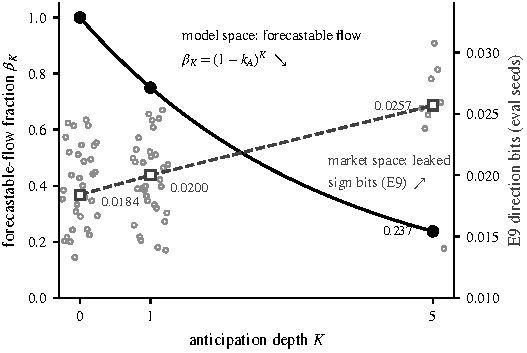
\includegraphics[width=0.78\linewidth]{deca3_inversion}
\caption{The inversion. Solid curve and filled circles (left axis): the
forecastable-flow fraction $\beta_K$ measured on the deterministic toy world,
falling exactly as $(1-k_A)^K$ --- $1.000 \to 0.750 \to 0.237$. Dashed line and
open squares (right axis): the E9 direction bits measured in the simulated
market at the same $K$ (open circles: the 8 evaluation seeds), medians
rising $0.0184 \to 0.0200 \to 0.0257$; the $K{=}5$ rise holds on 7 of 8
paired seeds. The operator removes forecastable
flow in model space; the market re-creates sign information in price space.
Open-loop contraction does not survive closed-loop equilibrium.}
% src: research/decathlon3.json forecastable_flow_fraction_vs_K, dir_bits_vs_K
\label{fig:inversion}
\end{figure}

Table~\ref{tab:deca3} and Figure~\ref{fig:inversion} give the result, which is
the paper's centerpiece. The kill criterion fires again, and this time the two
diagnostics move in \emph{opposite directions}: as $K$ goes $0 \to 1 \to 5$,
the model-space forecastable flow falls $1.000 \to 0.750 \to 0.237$ while the
market-space sign leak rises $0.0184 \to 0.0200 \to 0.0257$ bits in the
medians, with $K{=}5$ above the control on 7 of 8 paired seeds. The frozen
$K{=}5$ stack is moreover a two-event regression: its aggregate unwind adds
reversal (AC$_1$: $-0.075 \to -0.247$, breaking E1) and it absorbs the very
spiral that generates the leverage effect (E5 dies, $-0.095 \to -0.030$),
while tails erode (kurtosis $6.8 \to 5.3$) and crash asymmetry collapses (tail
ratio $44.8 \to 4.3$). Rational front-running at depth does not merely fail to
buy the missing events; at carry-over strength it kills wild facts the market
already had.
% src: research/decathlon3.json configs K1_DECA2/K5_FIXEDPOINT median_stats

The regression triggered the pre-registered contingent pass: six candidates on
disjoint tuning seeds came back 5/10 at best, tied across the three weakest
settings, and the pre-declared tie-break again selected the weakest ---
$k_A = 0.05$, an effective stack strength of $1 - 0.95^5 = 0.226$,
\emph{weaker than Experiment~I's single frozen layer} (0.25). Read once on the
evaluation seeds: 5/10, failing exactly the control's five events. The
selection pattern of Experiment~I repeats one level up: the battery pays for
less anticipation at every opportunity, never more.
% src: research/decathlon3.json tuning (grid, note), tuned_eval; docs/design/DESIGN20.md amendment

The algebra explains the failure sharply. Away from the caps, the $K$-layer
stack is equivalent to \emph{one} anticipator of strength $1-(1-k_A)^K$
(the telescoped sum in Eq.~\eqref{eq:stack}):
mutual anticipation of this operator class deepens into a stronger single
anticipator, and Experiment~I already measured that stronger is worse. The
contraction that defines the fixed point is an open-loop property, licensed by
the gate against an exogenous tape; it does not survive closed-loop
equilibrium, because every layer's inventory is a function of the same slow
public volatility state, so the stack's own price impact regenerates exactly
the forecastable structure the model says it removes. Model-space forecastable
flow down, market-space sign leak up: this is the cleanest statement we
know of why rational-expectations arguments cannot be reached by stacking
boundedly-capitalized flow traders.
% src: docs/FINDINGS.md DECATHLON-3 (mechanism paragraph)

\section{Experiment III: price-setting rationality}
\label{sec:deca4}

\subsection{The quote-skewing maker}

Experiments I and II killed every agent that \emph{trades} against the
forecastable flow: an anticipator's inventory rides the same slow public
state, so its trades re-leak what they absorb. One hypothesis survives that
diagnosis: price-\emph{setting} rationality --- a market maker who does not
trade but quotes, pre-adjusting the price by the expected impact of the
forecastable flow so that the information is absorbed into the price
\emph{level} rather than left in the return. The maker reuses the same causal
public-state forecast $\hat F_t$ of Eq.~\eqref{eq:forecast}, holds no
inventory, posts no flow, and draws no noise:
%
\begin{equation}
q_t = \lambda_Q\,\lambda\,\hat F_t, \qquad
r_t = \lambda\,D_t + (q_t - q_{t-1}),
\end{equation}
%
with $D_t$ the total flow in brackets in Eq.~\eqref{eq:market} and skew
strength $\lambda_Q \in \{1.0, 0.5\}$ fixed in advance
($\lambda_Q = 0$ is byte-identical to the unmodified simulator). Because the
maker's forecast state \emph{is} the targeters' public state, the quote
revision telescopes exactly against the mechanical flow
$f^{\mathrm{mech}}_t = D^{\mathrm{vol}}_t$,
$q_t - q_{t-1} = -\lambda_Q\,\lambda\, f^{\mathrm{mech}}_t$: at full skew the
mechanical flow's entire price impact is absorbed into the level by algebraic
identity, not by tuning, and the realized return keeps only the unforecastable
flow surprise. Nothing is left that could re-leak --- no inventory, no unwind,
no cap, no execution noise. The flow itself still executes untouched; only
where its impact lands (level versus return) changes.
% src: docs/design/DESIGN22.md (maker spec, telescoping identity)

The mechanism gate verifies this to the identity on the deterministic toy
world: at $\lambda_Q = 1$ the leak estimator
$\mathrm{corr}(f^{\mathrm{mech}}_t, r_{t+1})$ collapses from $+0.66$ to
$-0.06$ while the mechanical-flow series itself is essentially unchanged ---
absorption into the level, not suppression of the flow. The registration
declared this the third and final attempt on the expectation line and included
a closure clause: if the star hypothesis is refuted at this budget, the 5/10
ceiling is declared structural for this model class and the line closes.
% src: research/decathlon4.json toy_leak_corr_vs_lambda (0.6575 -> -0.0583); docs/design/DESIGN22.md closure clause

\subsection{Result: absorption deletes the wildness, not the leak}

\begin{table}[t]
\centering\small
\begin{tabular}{llll}
\toprule
Config & Score & Failed events & E9 bits (median) \\
\midrule
\cfg{FCVM} (control)              & 5/10 & E3 E4 E7 E8 E9 & 0.0184 \\
\cfg{FCVM+Q}($\lambda_Q{=}1.0$) (theory case) & 1/10 & all but E6 & 0.0237 \\
\cfg{FCVM+Q}($\lambda_Q{=}0.5$)   & 3/10 & E1 E2 E3 E4 E7 E8 E9 & 0.0180 \\
\cfg{Q}($\lambda_Q{=}0.05$) (tuned, contingent pass) & 5/10 & E3 E4 E7 E8 E9 & 0.0176 \\
\bottomrule
\end{tabular}
\caption{Experiment III. Full skew removes the vol-targeters' forecastable
impact exactly, and the sign leak does not close --- it grows (0.0237,
higher than the control on 7 of 8 seeds) --- while the wild facts die.}
% src: research/decathlon4.json configs, dir_bits_vs_lambda, contingent_pass
\label{tab:deca4}
\end{table}

\begin{figure}[t]
\centering
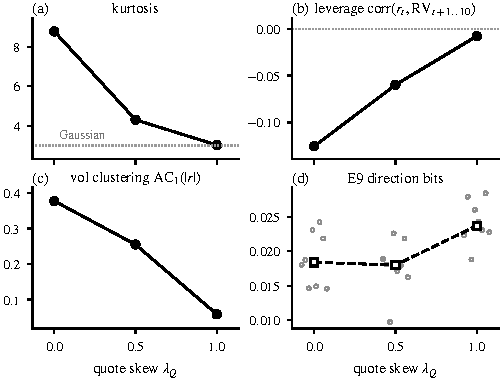
\includegraphics[width=0.78\linewidth]{deca4_wildfacts}
\caption{Wild-fact medians versus quote skew $\lambda_Q$ (8 evaluation seeds).
Full absorption of the forecastable flow's price impact kills the fat tails
(kurtosis $8.8 \to 3.0$), the leverage effect ($-0.125 \to -0.008$) and
volatility clustering (AC$_1(|r|)$ $0.38 \to 0.06$) --- while the E9 direction
bits (panel~d; open circles are seeds) do not close: flat at half skew,
higher at full skew.}
% src: research/decathlon4.json configs FCVM/FCVM+Q0.5/FCVM+Q1.0 median_stats, dir_bits_vs_lambda
\label{fig:wildfacts}
\end{figure}

Table~\ref{tab:deca4} and Figure~\ref{fig:wildfacts} give the sharpest
refutation of the three. The full-skew maker removes the vol-targeters'
forecastable impact exactly --- and the sign leak does not close. Bits stay
flat at half skew (0.0180 versus 0.0184) and \emph{grow} at full skew (0.0237,
higher than the control on 7 of 8 seeds). The leak was never the
vol-targeters' drift alone: Experiment~I's original attribution is overturned.
It lives distributed across \emph{all} the state-riding flows --- chartist
momentum, fundamentalist reversion, the one-lag maker's partial absorption ---
and deleting the spiral's impact strips away the wildness that was masking
them: efficiency breaks (AC$_1$: $+0.04 \to -0.26$; with the spiral gone the
liquidity provider's reversion dominates), and the newly-Gaussian returns make
the remaining structure easier to detect.
% src: research/decathlon4.json configs FCVM+Q1.0 median_stats; dir_bits per_seed comparison

The second pre-registered hypothesis --- that the maker would neutralize only
the forecastable \emph{mean} of the flow, leaving the volatility dynamics
intact --- is also refuted at the theory case, and its refutation is the
paper's central fact: in this market the forecastable flow \emph{is} the
wildness generator. Full absorption kills the fat tails (kurtosis
$8.8 \to 3.0$), the leverage effect ($-0.125 \to -0.008$), crash asymmetry
(tail ratio $40 \to 1.1$) and volatility clustering (AC$_1(|r|)$
$0.38 \to 0.06$) in one stroke. Half skew regresses too (3/10), so the
contingent pass fired: the six-candidate ladder came back flat at 5/10 for
every $\lambda_Q \le 0.30$, and the pre-declared weakest-skew tie-break picked
$\lambda_Q = 0.05$ --- the same selection pattern a third time, now for a
pricing rule. Read once on the evaluation seeds: 5/10, failing exactly the
control's five events. The battery pays for the least rationality at every
opportunity, in every agent class.
% src: research/decathlon4.json configs, contingent_pass (grid, winner_lambda, tuned_eval)

\begin{figure}[t]
\centering
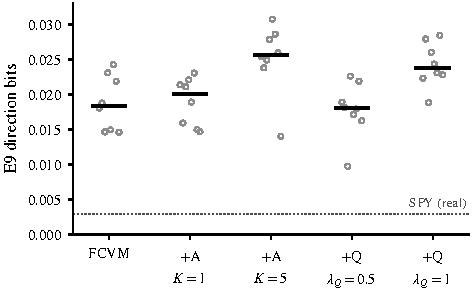
\includegraphics[width=0.78\linewidth]{e9_bits_configs}
\caption{E9 direction bits across every rationality configuration (open
circles: evaluation seeds; bars: medians). No configuration approaches the
information-free regime; real SPY (dotted, 0.0029) sits far below all of
them. Trading against the flow, iterating that trade to depth five, and
absorbing the flow's impact into the price level all leave the sign channel
open or wider.}
% src: research/decathlon3.json dir_bits_vs_K; research/decathlon4.json dir_bits_vs_lambda; research/decathlon.json spy.stats.dir_bits
\label{fig:bits}
\end{figure}

Figure~\ref{fig:bits} collects the E9 evidence across all three experiments.

\section{The structural claim and its limits}
\label{sec:structural}

\subsection{The closure clause as methodology}

Experiment III's registration contained, alongside its hypotheses and budget,
a closure clause: this is the third and final attempt on the expectation line;
if the star hypothesis is refuted at this budget, the 5/10 ceiling is declared
structural for flow-based minimal markets with boundedly-rational agents of
every class here considered, and the line closes --- no fourth experiment. The
clause is not rhetoric; it is the instrument that converts three negative
results into one positive claim. An open-ended sequence of failed attempts
supports only ``we have not yet found the right agent.'' A pre-committed final
attempt, refuted, supports a stronger statement about the class that was
searched --- precisely because the search was budgeted, the budget was spent,
and the stopping rule was declared before the last result was known.
% src: docs/design/DESIGN22.md closure clause; docs/FINDINGS.md DECATHLON-4

\subsection{The claim}

The three refutations compose. In this model class, the forecastable flow
component and the wild one-sided facts are the same object:
%
\begin{enumerate}
\item an agent who \emph{trades} against the forecastable flow adds its own
  forecastable flow, because its inventory rides the same slow public state
  --- the leak moves one derivative earlier (Experiment~I);
\item stacking such agents to the fixed point of mutual anticipation is
  algebraically one stronger such agent, and re-leaks harder while the
  model-space forecastable flow contracts to 0.237 (Experiment~II);
\item a price-setter who absorbs the flow's impact exactly --- the
  rational-expectations limit for this channel, verified to the identity ---
  can close the leak only by deleting the de-leveraging dynamics that generate
  the tails, the leverage effect, and the crash asymmetry, scoring 1/10
  (Experiment~III).
\end{enumerate}
%
Sign-efficiency and wildness are not separate dials: in a market moved by
state-riding flows they are jointly produced, and no bolt-on layer of
rationality --- trading, iterated, or price-setting --- buys the five missing
events (E3, E4, E7, E8, E9). What the minimal market lacks is not a smarter
agent but a different kind of memory: the long-memory clock and the coupling
arrow live upstream of the flows, in whatever generates them.
% src: docs/FINDINGS.md DECATHLON-4 (closure paragraph)

\subsection{What is explicitly not claimed}

The claim is scoped, and the scoping is part of the result. Explicitly
\emph{not} claimed: anything about real markets' generating process; anything
beyond this model class (no learning agents, no heterogeneous information, no
strategic equilibrium or rational-expectations solution concept); optimality
of the agent designs --- each is gate-verified to \emph{function}, not to be
optimal.
% src: docs/paper/OUTLINE.md (NOT-claimed list, near-verbatim)

``Structural'' here means: invariant over the searched class under the
pre-registered budgets, with each searched member licensed by a mechanism gate
proving it expresses its hypothesis. The claim would be falsified by an agent
class outside the three --- learning agents that condition on more than the
public volatility state, or information-heterogeneous agents whose inventories
do not ride a common public state --- breaking the ceiling under the same
battery and the same protocol. That is an open door, and we name it as such
rather than hedge the claim through it.

\section{Empirical counterpart: the microstructure triangle}
\label{sec:triangle}

The model mechanism makes the wildness channel a property of the \emph{flow
structure}: the leverage effect in the minimal market exists because a
one-directional, state-riding de-leveraging flow exists, and dies when that
flow's impact is removed (Figure~\ref{fig:wildfacts}). A weak but testable
empirical counterpart: across real asset classes, the leverage effect should
follow the microstructure that does or does not host such flows.

\begin{figure}[t]
\centering
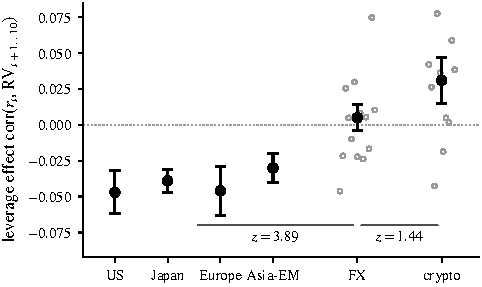
\includegraphics[width=0.8\linewidth]{leverage_triangle}
\caption{The leverage effect
$\mathrm{corr}(r_t, \mathrm{RV}_{t+1..10})$ at three microstructure vertices.
Filled points: cohort estimates $\pm$1 s.d. Open circles: the 13 individual FX
crosses and 10 individual coins. Equities (four universes: US, Japan, Europe,
Asia-EM) sit at $-0.030$ to $-0.047$; FX at $+0.005 \pm 0.009$ (statistically
zero, $z = 0.56$); crypto at $+0.031 \pm 0.016$. The equity--FX separation is
resolved ($z = 3.89$); the FX--crypto separation is not ($z = 1.44$).}
% src: research/fx.json laws.leverage, leverage_contrast, per_pair_leverage; research/crypto.json per_coin_leverage
\label{fig:triangle}
\end{figure}

\begin{table}[t]
\centering\small
\begin{tabular}{lccc}
\toprule
 & equity cohort & FX & crypto \\
\midrule
leverage effect & $-0.0405 \pm 0.0079$ & $+0.005 \pm 0.009$ & $+0.031 \pm 0.016$ \\
$z$ vs.\ zero & $-5.1$ & 0.56 & 1.97 \\
$z$ vs.\ FX & 3.89 & --- & 1.44 \\
instruments positive & 0 of 4 markets & 7 of 13 pairs & 8 of 10 coins \\
\bottomrule
\end{tabular}
\caption{The leverage triangle. Equity cohort: four universes (US, Japan,
Europe, Asia-EM), 2010--2026. FX: 13 liquid crosses, 2010--2026. Crypto: 10
major coins, 2017--2026. Each $z$ vs.\ zero is the cohort mean divided by its
cross-sectional dispersion (the $\pm$ values in the first row). The ordering
$-0.041 < +0.005 < +0.031$ is monotone in point estimates; the equity edge is
statistically certified, the FX--crypto edge is inside one-sided noise.}
% src: research/fx.json leverage_contrast (equity_mean, equity_spread, fx_leverage, fx_sd, z_fx_vs_zero, z_fx_vs_equities, z_crypto_vs_fx), n_pairs_positive; research/crypto.json leverage_contrast, per_coin_leverage
% src: z-vs-zero equity and crypto DERIVED as mean/sd from the stored fields: equity_mean/equity_spread = -0.0405/0.0079 = -5.13; crypto_leverage/crypto_sd = 0.0312/0.0158 = 1.97 (crypto.json); checked by docs/paper/check_numbers.py
\label{tab:triangle}
\end{table}

Table~\ref{tab:triangle} and Figure~\ref{fig:triangle} give the measurement,
using an estimator battery identical across the three vertices (realized
variance from daily OHLC ranges via Garman--Klass \citep{garman1980}). The
classical readings of the equity effect --- firm capital structure
\citep{black1976} and volatility feedback through the equity risk premium
\citep{bekaert2000} --- are equity-specific mechanisms, which is exactly what
makes the cross-venue comparison informative: a currency is not a levered
claim and carries no equity premium, so whatever asymmetry survives outside
equities must come from the venue's flow structure. Equity markets
--- where financial leverage and institutional de-risking cascades live ---
show the textbook negative effect in all four universes ($-0.030$ to
$-0.047$). FX --- an institutional dealer market hosting neither de-risking
cascades nor a dominant retail-momentum dynamic --- is
statistically zero ($+0.005$, $z$ vs.\ zero $= 0.56$; 7 of 13 pairs positive,
the symmetric scatter a true zero predicts). Crypto --- no financial leverage,
no institutional de-risking, a retail dynamic in which rallies rather than
crashes spike volatility --- sits at $+0.031$, with 8 of 10 coins individually
positive and only BTC ($-0.043$) and ETH ($-0.019$) retaining the equity-style
sign.
% src: research/fx.json laws.leverage.values, per_pair_leverage; research/crypto.json per_coin_leverage

Honesty about what is certified: the equity edge is resolved (one-sided
$z = 3.89$ against FX, $z = 4.06$ against crypto), and FX is decisively zero;
but the FX--crypto edge is $z = 1.44$, inside noise, and crypto itself clears
zero at only $z \approx 2$ --- so ``crypto genuinely positive above an FX
zero'' is an ordering of point estimates, not a certified separation. The
residual per-pair scatter in FX lies on the flight-to-quality axis: the three
most negative crosses are all yen pairs (AUDJPY $-0.046$, GBPJPY $-0.024$,
EURJPY $-0.022$ --- yen strength is risk-off, so ``down $\to$ vol up'' is
flight-to-quality wearing leverage's clothes), and the most positive is USDMXN
($+0.075$, the same flow with the opposite quote orientation).
% src: research/crypto.json leverage_contrast.z_vs_equities; research/fx.json leverage_contrast, per_pair_leverage

The reading is licensed by a sign-recovery gate: on synthetic worlds with a
known leverage sign (equity-negative, inverted-positive, symmetric-zero), the
estimator recovers each with wide separation and its spurious-leverage bound
is $|0.04|$, so a zero is read as a zero and an inversion as an inversion.
% src: docs/FINDINGS.md KRONOS-CRYPTO (gate X26), KRONOS-FX (spurious bound)

The positioning is deliberate: this triangle is \emph{consistent with} the
thesis --- the wildness channel follows the flow structure of the venue, being
negative exactly where forced de-risking lives, zero in the institutional
market without it, and (in point estimate) positive where an opposite retail
dynamic dominates --- but it is not proof of it. No claim is made that the
minimal market's specific mechanism generates the real effect.

\section{Related work}
\label{sec:related}

\citet{cont2001} fixed the stylized-facts target list this battery
operationalizes; our contribution to that program is calibration at both ends
(real data 10/10, GBM exactly 3/10) so that partial scores are interpretable.
The agent-based literature descending from \citet{lux1999} and surveyed by
\citet{lebaron2006} established that fundamentalist--chartist interaction
buys fat tails and clustering; our ablation reproduces that result (and its
fragility: chartists without market makers destroy efficiency, scoring 1/10)
but differs in asking the complement --- which facts a flow-based market
\emph{cannot} buy at any rationality depth, established by pre-registered
refutation rather than by exhibition.
% src: research/decathlon.json configs.FC.score

Two adjacent traditions ask closely related questions with different
instruments. In the heterogeneous-beliefs models of \citet{brock1998},
the sophistication of agents' expectations is a bifurcation parameter of a
deterministic pricing map: making agents more forward-looking changes the
dynamics qualitatively rather than monotonically improving them. Our
$K$-ladder is a stochastic, capital-bounded cousin of that exercise, and it
finds the same non-monotonicity in a measured quantity --- the sign leak
grows as anticipation deepens. The minority-game literature
\citep{challet1997} and the intermittent agent-based markets of
\citet{giardina2003} derive stylized facts from the statistical mechanics of
adaptive agents competing over a scarce resource, with realistic regimes
appearing near phase boundaries; our battery differs in scoring a fixed list
of calibrated events rather than exhibiting a regime, but the joint-production
finding rhymes with that literature's lesson that efficiency and excess
volatility are properties of one collective state, not separate features.

The paper's E9 event operationalizes the oldest target in the field.
\citet{samuelson1965} proved that properly anticipated prices fluctuate
randomly; \citet{fama1970} organized the empirical program around
informational efficiency; and \citet{grossman1980} showed that full
informational efficiency is impossible when information is costly --- an
equilibrium amount of inefficiency must survive to pay the agents who remove
it. The joint-production result is a mechanical relative of that
impossibility with the cost relocated: in this model class the residual sign
information is not a fee paid to arbitrageurs but a by-product of the same
state-riding flows that generate the volatility structure, and the three
experiments show it cannot be traded, iterated, or quoted away without taking
the wildness with it.

The price-impact literature of Bouchaud and coauthors
\citep{bouchaud2009, bouchaud2018} underlies the paper's central object: the
idea that order flow is the proximate mover of prices and that liquidity
provision digests predictable flow. Our quote-skewing maker is a minimal
formalization of perfect digestion --- and Experiment~III's finding that exact
absorption deletes the volatility dynamics along with the leak is, in that
vocabulary, a statement that the market's wildness \emph{is} its undigested
flow. \citet{filimonov2012} measured near-critical reflexivity in markets via
the Hawkes branching ratio; the measurement program behind this paper found
that result replicates raw (branching ratio $0.68$ across 48 US assets) but
collapses to $0.25$ --- a no-self-excitation null --- once events are deformed
by the volatility clock, so most apparent reflexivity at the daily horizon is
volatility clustering; the same deformation-first discipline shapes the
battery's E8 event.
% src: research/reflex.json median_n_raw=0.6827, median_n_def=0.2459, per_asset (48 assets); docs/FINDINGS.md KRONOS-REFLEX
Rough volatility \citep{gatheral2018} motivates the battery's long-memory
clock event E4: the measurement program replicated a Hurst exponent
$H \approx 0.10$ on 16
years of SPY range-based volatility, and E4 is calibrated so that
exponential-memory processes (GJR-GARCH) fail it --- which is exactly the
event no flow configuration and no rationality layer ever bought, consistent
with rough volatility's message that the clock's memory is structural, not
flow-generated.
% src: research/rough.json daily.H=0.1013; docs/design/DESIGN8.md amendment 1 (GJR fails E4)

\section{Methods}
\label{sec:methods}

\subsection{Convict-and-exonerate gates}

\begin{figure}[t]
\centering
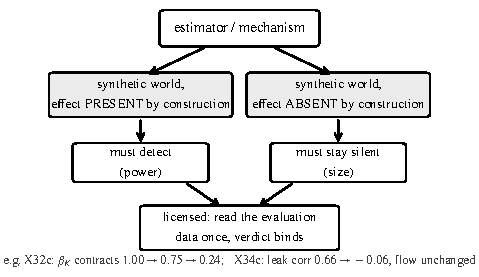
\includegraphics[width=0.7\linewidth]{gate_schematic}
\caption{The gate pattern. Every estimator and every tested mechanism must,
before any evaluation data is read, both detect a planted effect on a
synthetic world where the effect exists (power) and stay silent on a world
where it does not (size). The examples are this paper's: the fixed-point
operator's contraction gate and the quote-skew maker's absorption gate.}
% src: docs/METHODS.md section 0; research/decathlon3.json forecastable_flow_fraction_vs_K; research/decathlon4.json toy_leak_corr_vs_lambda
\label{fig:gate}
\end{figure}

Every estimator in the program passes a gate before touching evaluation data:
a test on synthetic data where the answer is known, proving both size (on a
world where the effect is absent, the test does not fire) and power (on a
world where the effect is present by construction, it does)
(Figure~\ref{fig:gate}). The battery's estimators were licensed this way
before the first agent-based run, and --- the step specific to this paper ---
so was every \emph{tested mechanism}: the anticipator was proven to profit and
damp flow impact on a toy world (Section~\ref{sec:deca2}), the fixed-point
stack to contract forecastable flow (Section~\ref{sec:deca3}), the
quote-skewing maker to absorb impact while leaving the flow untouched
(Section~\ref{sec:deca4}). This is what makes the refutations evidential:
when a licensed mechanism fails to move the battery, the failure is a property
of the market, not of a broken implementation. At the time of writing the
continuous-integration suite runs the numbered gates X1--X35 on every commit.
% src: tests/*.py (gate identifiers X1..X35, verified by grep); docs/METHODS.md sections 0 and 8

\subsection{Pre-registration, budgets, and tie-breaks}

``Pre-registered'' here means: the design document --- hypotheses, budgets,
kill criteria --- is committed to the repository before any evaluation run,
and the version-control history is the timestamp; there is no external
registry. Each experiment fixed, before any evaluation run: hypotheses (with
one starred primary), the full parameter set, the evaluation protocol (8
seeds, IDs 100--107, $T = 6000$, majority vote per event, identical across
all three experiments so ablations are paired seed-for-seed), a kill
criterion, and a bounded tuning budget --- one grid pass on disjoint tuning seeds (900--903), permitted
only under a pre-declared trigger, with a deterministic pre-declared tie-break
(``weakest intervention wins''). Amendments were permitted only before
evaluation data was read, and each is recorded in the registration documents
with its trigger. Two facts about this protocol did real work. First, the
kill criteria fired three times and were honored three times. Second, the
tie-break rule turned the tuning passes themselves into evidence: in all three
experiments the battery's preferred setting was the weakest intervention
available --- the market scores best when the rational agent barely acts ---
which is the structural claim visible in the selection pattern before it is
visible in the scores.
% src: docs/design/DESIGN18.md, DESIGN20.md, DESIGN22.md (budgets, amendments); research/decathlon{2,3,4}.json tuning blocks

\subsection{Reproducibility discipline}

Three practices matter for the trustworthiness of small numeric differences.
(1) \emph{Byte-identity pins}: every new mechanism ships behind a flag, and a
gate asserts that flag-off output is byte-identical to the pre-change
simulator, so the calibration (SPY 10/10, GBM 3/10) and all previously
published rows are protected across the entire arc; Experiment~II's $K{=}1$
reproduces Experiment~I's published configuration exactly, and Experiment
III's $\lambda_Q{=}0$ reproduces both. (2) \emph{Causality gates}: tampering
with future inputs must leave the trade or quote prefix bit-identical (and the
tail must differ, proving the mechanism actually reads the tape). (3)
\emph{Architecture-portable assertions}: an early version of the pins asserted
absolute byte hashes of floating-point output, which held on one CPU
architecture and failed on another by units in the last place; the discipline
that survives is to assert in-process equivalence and architecture-stable
invariants rather than absolute hashes.
% src: docs/design/DESIGN20.md, DESIGN22.md (gates X32a, X34a); docs/METHODS.md §0 (arch-dependent-pin lesson)

Separately from this paper's claims: performance claims elsewhere in the same
research program are governed by a trial ledger and reported as deflated
Sharpe ratios \citep{bailey2014} beside a combinatorially cross-validated
probability of backtest overfitting \citep{bailey2017}; the program's standing
rule is that its PBO of 0.45 is restated beside any Sharpe claim. This paper
makes mechanism claims, not performance claims, but the same accounting
culture --- count the shots, publish the misses --- produced it.
% src: research/forensics.json pbo.pbo=0.4455; docs/METHODS.md sections 5 and 8; docs/FINDINGS.md (PBO 0.45 standing rule)

\subsection{Code and data availability}
\label{sec:repro}

Every number in this paper is regenerable from the public repository. The
research JSONs consumed by the figures and tables ---
\texttt{decathlon.json}, \texttt{decathlon2.json}, \texttt{decathlon3.json},
\texttt{decathlon4.json}, \texttt{fx.json} and \texttt{crypto.json}, all
under \texttt{research/} --- are versioned in the repository and rebuilt by
\texttt{run\_research.py}; the battery code is identical for real data and
simulated output; the gate suite runs in continuous integration on every
commit, including the byte-identity pins that protect every published row in
this paper; and all six figures are generated from the research JSONs by
\texttt{docs/paper/make\_figures.py} with no hand-entered values. The
pre-registration documents, including the amendments and the closure clause
quoted here, are versioned in \texttt{docs/design/}.

\appendix

\section{The battery: exact criteria and calibration statistics}
\label{app:battery}

Table~\ref{tab:thresholds} states each event's statistic and pass region
exactly as
implemented in the repository (\texttt{kronos/decathlon.py}, function
\texttt{battery}; the thresholds were fixed in the DESIGN8 registration and
its calibration-phase amendments), and Table~\ref{tab:calib} gives the full
statistic vector at both calibration ends and at the flow-only ceiling.
Notation: $r_t$ are daily returns;
$\mathrm{RV}_t$ is the 5-day rolling mean of $r^2$ (the close-only volatility
clock), $\sigma_t = \sqrt{\mathrm{RV}_t}$ (written $\sigma_{5d}$ in
Table~\ref{tab:events}), and $z_t = r_t/\sigma_t$ the
deformed (one-clock) return. The weekly clock is built from
\emph{non-overlapping} 5-day means $w_j$ of $\log r^2$ --- raw weekly
differences carry an MA(1) artifact on which even GBM's $|\Delta w|$
autocorrelates, so E4 uses the level and E7 uses AR(1) innovations
$u_j = w_{j+1} - \bar w(1-\phi) - \phi w_j$ with $\phi$ the fitted AR(1)
coefficient. $\mathrm{AC}_k(\cdot)$ is the lag-$k$ autocorrelation.
A configuration passes an event if a majority of its 8 evaluation seeds pass.
% src: kronos/decathlon.py battery(), weekly_clock_stats(); docs/design/DESIGN8.md amendments

\begin{table}[t]
\centering\small
\begin{tabular}{llp{6.1cm}}
\toprule
\# & Statistic & Pass region \\
\midrule
E1 & $\mathrm{AC}_1(r)$ & $[-0.15,\ 0.05]$ \\
E2 & kurtosis$(r)$ & $[4.5,\ 40]$ \\
E3 & $\mathrm{AC}_1(|r|)$ and $\mathrm{mean}_{k=5..20}\,\mathrm{AC}_k(|r|)$ & $\ge 0.12$ and $\ge 0.05$ \\
E4 & $\mathrm{AC}_8(w)$ (weekly clock level) & $\ge 0.12$ \\
E5 & $\mathrm{mean}_{\tau=1..10}\,\mathrm{corr}(r_t, \mathrm{RV}_{t+\tau})$ & $\le -0.03$ \\
E6 & kurtosis$(z)$ & $\le 5$ \\
E7 & skew$(u)$ (weekly clock AR(1) innovations) & $\ge -0.35$ \\
E8 & $\mathrm{EP}(r)$, $\mathrm{EP}(z)$ (entropy production, bits) & $\mathrm{EP}(r)$ significant and $\mathrm{EP}(z) \le 0.75\,\mathrm{EP}(r)$ \\
E9 & direction bits $I(\text{features};\, \mathrm{sign}\, r_{t+1})$ & $\le$ 95th percentile of 120 shuffles \\
E10 & $\#\{r < -2.5 s\} \,/\, \#\{r > +2.5 s\}$, $s = \mathrm{sd}(r)$ & $\ge 1.25$ \\
\bottomrule
\end{tabular}
\caption{Exact pass criteria, as implemented. E7's floor is calibrated
against the log-$\chi^2$ noise skew of the weekly clock (GBM innovations skew
$\approx -0.65$; real SPY $-0.22$). E8's entropy production symbolizes the
series into 3 bins, measures 3-gram irreversibility, and tests against 120
block-reversal surrogates (random block offsets, blocks reversed with
probability $1/2$). E9's features are the Cartesian product of three tape
observables --- $\mathrm{sign}(r_t)$, the sign of 21-day momentum, and the
volatility tercile --- scored by discrete plug-in mutual information with
Miller--Madow bias correction against a 120-permutation null; the program's
continuous information channel uses the KSG estimator \citep{kraskov2004},
but E9's features are discrete by construction. The volatility tercile is cut
on full-sample quantiles: E9 is a measurement of information content,
computed identically on real and simulated series, not a trading rule.}
% src: kronos/decathlon.py battery(); kronos/entropyprod.py ep_with_null(); kronos/infobudget.py direction_bits()
\label{tab:thresholds}
\end{table}

\begin{table}[t]
\centering\small
\begin{tabular}{llrrr}
\toprule
Statistic & Event & SPY (real) & GBM (G) & \cfg{FCVM} \\
\midrule
$\mathrm{AC}_1(r)$            & E1  & $-0.103$ & $0.001$  & $0.036$ \\
kurtosis$(r)$                 & E2  & $15.09$  & $3.04$   & $8.79$ \\
$\mathrm{AC}_1(|r|)$          & E3  & $0.307$  & $-0.001$ & $0.377$ \\
mean $\mathrm{AC}_{5..20}(|r|)$ & E3 & $0.218$  & $0.002$  & $-0.050$ \\
$\mathrm{AC}_8(w)$            & E4  & $0.186$  & $-0.018$ & $-0.003$ \\
leverage                      & E5  & $-0.113$ & $0.007$  & $-0.125$ \\
kurtosis$(z)$                 & E6  & $2.33$   & $2.13$   & $2.20$ \\
skew$(u)$                     & E7  & $-0.221$ & $-0.651$ & $-0.408$ \\
$\mathrm{EP}(r)$ bits         & E8  & $0.0211$ & $0.0002$ & $0.0929$ \\
$\mathrm{EP}(z)$ bits         & E8  & $0.0141$ & $0.0006$ & $0.1392$ \\
direction bits                & E9  & $0.0029$ & $0.0001$ & $0.0184$ \\
tail asymmetry                & E10 & $1.56$   & $0.91$   & $39.96$ \\
\bottomrule
\end{tabular}
\caption{The full statistic vector at the battery's calibration ends (SPY
10/10, GBM 3/10) and at the flow-only ceiling (\cfg{FCVM}, 5/10); GBM and
\cfg{FCVM} entries are medians over the 8 evaluation seeds. The table shows
\emph{how} each score decomposes: GBM passes only E1, E6, E9; \cfg{FCVM}
matches SPY's magnitudes on E1/E2/E5/E10 but has no clock memory
($\mathrm{AC}_8(w)\approx 0$ against SPY's $0.186$), fails E8 on the ratio
criterion ($\mathrm{EP}(z) > 0.75\,\mathrm{EP}(r)$: deformation does not
reduce its entropy production), and leaks $6\times$ SPY's direction bits.
Its E7 skew ($-0.408$) sits marginally below the $-0.35$ floor. SPY's
$\mathrm{EP}(z)$ is significant but 33\% below $\mathrm{EP}(r)$, meeting the
ratio criterion.}
% src: research/decathlon.json spy.stats, configs.G.median_stats, configs.FCVM.median_stats
\label{tab:calib}
\end{table}

Two calibration facts anchor the thresholds. GBM's weekly-clock innovation
skew ($-0.651$) is the log-$\chi^2$ noise floor E7 is calibrated against;
real volatility's up-jumps cancel most of it (SPY $-0.221$). And the E4
level-autocorrelation criterion is what a GJR-GARCH process fails (clock
$\mathrm{AC}_8 \approx 0.06$ against the $0.12$ bar): exponential memory
decays too fast at eight weeks, which is why E4 is the battery's long-memory
event rather than any Hurst point estimate (the close-only Hurst proxy is
biased and is recorded as informational only).
% src: docs/design/DESIGN8.md amendment 1; kronos/decathlon.py comments (E4, E7)

\begin{thebibliography}{17}

\bibitem[Bailey and L{\'o}pez de Prado(2014)]{bailey2014}
Bailey, D.~H., and M.~L{\'o}pez de Prado (2014).
The deflated Sharpe ratio: Correcting for selection bias, backtest
overfitting, and non-normality.
\emph{Journal of Portfolio Management}, 40(5), 94--107.

\bibitem[Bailey et~al.(2017)]{bailey2017}
Bailey, D.~H., J.~Borwein, M.~L{\'o}pez de Prado, and Q.~J. Zhu (2017).
The probability of backtest overfitting.
\emph{Journal of Computational Finance}, 20(4), 39--69.

\bibitem[Bekaert and Wu(2000)]{bekaert2000}
Bekaert, G., and G.~Wu (2000).
Asymmetric volatility and risk in equity markets.
\emph{Review of Financial Studies}, 13(1), 1--42.

\bibitem[Black(1976)]{black1976}
Black, F. (1976).
Studies of stock price volatility changes.
In \emph{Proceedings of the 1976 Meetings of the American Statistical
Association, Business and Economic Statistics Section}, 177--181.

\bibitem[Bouchaud et~al.(2009)]{bouchaud2009}
Bouchaud, J.-P., J.~D. Farmer, and F.~Lillo (2009).
How markets slowly digest changes in supply and demand.
In T.~Hens and K.~R. Schenk-Hopp{\'e} (eds.),
\emph{Handbook of Financial Markets: Dynamics and Evolution}, North-Holland.

\bibitem[Bouchaud et~al.(2018)]{bouchaud2018}
Bouchaud, J.-P., J.~Bonart, J.~Donier, and M.~Gould (2018).
\emph{Trades, Quotes and Prices: Financial Markets Under the Microscope}.
Cambridge University Press.

\bibitem[Brock and Hommes(1998)]{brock1998}
Brock, W.~A., and C.~H. Hommes (1998).
Heterogeneous beliefs and routes to chaos in a simple asset pricing model.
\emph{Journal of Economic Dynamics and Control}, 22(8--9), 1235--1274.

\bibitem[Challet and Zhang(1997)]{challet1997}
Challet, D., and Y.-C. Zhang (1997).
Emergence of cooperation and organization in an evolutionary game.
\emph{Physica A}, 246(3--4), 407--418.

\bibitem[Cont(2001)]{cont2001}
Cont, R. (2001).
Empirical properties of asset returns: Stylized facts and statistical issues.
\emph{Quantitative Finance}, 1(2), 223--236.

\bibitem[Fama(1970)]{fama1970}
Fama, E.~F. (1970).
Efficient capital markets: A review of theory and empirical work.
\emph{Journal of Finance}, 25(2), 383--417.

\bibitem[Filimonov and Sornette(2012)]{filimonov2012}
Filimonov, V., and D.~Sornette (2012).
Quantifying reflexivity in financial markets: Toward a prediction of flash
crashes.
\emph{Physical Review E}, 85(5), 056108.

\bibitem[Garman and Klass(1980)]{garman1980}
Garman, M.~B., and M.~J. Klass (1980).
On the estimation of security price volatilities from historical data.
\emph{Journal of Business}, 53(1), 67--78.

\bibitem[Gatheral et~al.(2018)]{gatheral2018}
Gatheral, J., T.~Jaisson, and M.~Rosenbaum (2018).
Volatility is rough.
\emph{Quantitative Finance}, 18(6), 933--949.

\bibitem[Giardina and Bouchaud(2003)]{giardina2003}
Giardina, I., and J.-P. Bouchaud (2003).
Bubbles, crashes and intermittency in agent based market models.
\emph{European Physical Journal B}, 31(3), 421--437.

\bibitem[Grossman and Stiglitz(1980)]{grossman1980}
Grossman, S.~J., and J.~E. Stiglitz (1980).
On the impossibility of informationally efficient markets.
\emph{American Economic Review}, 70(3), 393--408.

\bibitem[Kraskov et~al.(2004)]{kraskov2004}
Kraskov, A., H.~St{\"o}gbauer, and P.~Grassberger (2004).
Estimating mutual information.
\emph{Physical Review E}, 69(6), 066138.

\bibitem[LeBaron(2006)]{lebaron2006}
LeBaron, B. (2006).
Agent-based computational finance.
In L.~Tesfatsion and K.~L. Judd (eds.),
\emph{Handbook of Computational Economics}, Vol.~2, North-Holland,
1187--1233.

\bibitem[Lux and Marchesi(1999)]{lux1999}
Lux, T., and M.~Marchesi (1999).
Scaling and criticality in a stochastic multi-agent model of a financial
market.
\emph{Nature}, 397(6719), 498--500.

\bibitem[Samuelson(1965)]{samuelson1965}
Samuelson, P.~A. (1965).
Proof that properly anticipated prices fluctuate randomly.
\emph{Industrial Management Review}, 6(2), 41--49.

\end{thebibliography}

\end{document}
